
%% bare_conf.tex
%% V1.3
%% 2007/01/11
%% by Michael Shell
%% See:
%% http://www.michaelshell.org/
%% for current contact information.
%%
%% This is a skeleton file demonstrating the use of IEEEtran.cls
%% (requires IEEEtran.cls version 1.7 or later) with an IEEE conference paper.
%%
%% Support sites:
%% http://www.michaelshell.org/tex/ieeetran/
%% http://www.ctan.org/tex-archive/macros/latex/contrib/IEEEtran/
%% and
%% http://www.ieee.org/

%%*************************************************************************
%% Legal Notice:
%% This code is offered as-is without any warranty either expressed or
%% implied; without even the implied warranty of MERCHANTABILITY or
%% FITNESS FOR A PARTICULAR PURPOSE! 
%% User assumes all risk.
%% In no event shall IEEE or any contributor to this code be liable for
%% any damages or losses, including, but not limited to, incidental,
%% consequential, or any other damages, resulting from the use or misuse
%% of any information contained here.
%%
%% All comments are the opinions of their respective authors and are not
%% necessarily endorsed by the IEEE.
%%
%% This work is distributed under the LaTeX Project Public License (LPPL)
%% ( http://www.latex-project.org/ ) version 1.3, and may be freely used,
%% distributed and modified. A copy of the LPPL, version 1.3, is included
%% in the base LaTeX documentation of all distributions of LaTeX released
%% 2003/12/01 or later.
%% Retain all contribution notices and credits.
%% ** Modified files should be clearly indicated as such, including  **
%% ** renaming them and changing author support contact information. **
%%
%% File list of work: IEEEtran.cls, IEEEtran_HOWTO.pdf, bare_adv.tex,
%%                    bare_conf.tex, bare_jrnl.tex, bare_jrnl_compsoc.tex
%%*************************************************************************

% *** Authors should verify (and, if needed, correct) their LaTeX system  ***
% *** with the testflow diagnostic prior to trusting their LaTeX platform ***
% *** with production work. IEEE's font choices can trigger bugs that do  ***
% *** not appear when using other class files.                            ***
% The testflow support page is at:
% http://www.michaelshell.org/tex/testflow/



% Note that the a4paper option is mainly intended so that authors in
% countries using A4 can easily print to A4 and see how their papers will
% look in print - the typesetting of the document will not typically be
% affected with changes in paper size (but the bottom and side margins will).
% Use the testflow package mentioned above to verify correct handling of
% both paper sizes by the user's LaTeX system.
%
% Also note that the "draftcls" or "draftclsnofoot", not "draft", option
% should be used if it is desired that the figures are to be displayed in
% draft mode.
%
\documentclass[conference]{IEEEtran}
% Add the compsoc option for Computer Society conferences.
%
% If IEEEtran.cls has not been installed into the LaTeX system files,
% manually specify the path to it like:
% \documentclass[conference]{../sty/IEEEtran}





% Some very useful LaTeX packages include:
% (uncomment the ones you want to load)


% *** MISC UTILITY PACKAGES ***
%
%\usepackage{ifpdf}
% Heiko Oberdiek's ifpdf.sty is very useful if you need conditional
% compilation based on whether the output is pdf or dvi.
% usage:
% \ifpdf
%   % pdf code
% \else
%   % dvi code
% \fi
% The latest version of ifpdf.sty can be obtained from:
% http://www.ctan.org/tex-archive/macros/latex/contrib/oberdiek/
% Also, note that IEEEtran.cls V1.7 and later provides a builtin
% \ifCLASSINFOpdf conditional that works the same way.
% When switching from latex to pdflatex and vice-versa, the compiler may
% have to be run twice to clear warning/error messages.






% *** CITATION PACKAGES ***
%
%\usepackage{cite}
% cite.sty was written by Donald Arseneau
% V1.6 and later of IEEEtran pre-defines the format of the cite.sty package
% \cite{} output to follow that of IEEE. Loading the cite package will
% result in citation numbers being automatically sorted and properly
% "compressed/ranged". e.g., [1], [9], [2], [7], [5], [6] without using
% cite.sty will become [1], [2], [5]--[7], [9] using cite.sty. cite.sty's
% \cite will automatically add leading space, if needed. Use cite.sty's
% noadjust option (cite.sty V3.8 and later) if you want to turn this off.
% cite.sty is already installed on most LaTeX systems. Be sure and use
% version 4.0 (2003-05-27) and later if using hyperref.sty. cite.sty does
% not currently provide for hyperlinked citations.
% The latest version can be obtained at:
% http://www.ctan.org/tex-archive/macros/latex/contrib/cite/
% The documentation is contained in the cite.sty file itself.






% *** GRAPHICS RELATED PACKAGES ***
%
\ifCLASSINFOpdf
  \usepackage[pdftex]{graphicx}
  % declare the path(s) where your graphic files are
  \graphicspath{{../pdf/}{../jpeg/}}
  % and their extensions so you won't have to specify these with
  % every instance of \includegraphics
  \DeclareGraphicsExtensions{.pdf,.jpeg,.png}
\else
  % or other class option (dvipsone, dvipdf, if not using dvips). graphicx
  % will default to the driver specified in the system graphics.cfg if no
  % driver is specified.
  % \usepackage[dvips]{graphicx}
  % declare the path(s) where your graphic files are
  % \graphicspath{{../eps/}}
  % and their extensions so you won't have to specify these with
  % every instance of \includegraphics
  % \DeclareGraphicsExtensions{.eps}
\fi
% graphicx was written by David Carlisle and Sebastian Rahtz. It is
% required if you want graphics, photos, etc. graphicx.sty is already
% installed on most LaTeX systems. The latest version and documentation can
% be obtained at: 
% http://www.ctan.org/tex-archive/macros/latex/required/graphics/
% Another good source of documentation is "Using Imported Graphics in
% LaTeX2e" by Keith Reckdahl which can be found as epslatex.ps or
% epslatex.pdf at: http://www.ctan.org/tex-archive/info/
%
% latex, and pdflatex in dvi mode, support graphics in encapsulated
% postscript (.eps) format. pdflatex in pdf mode supports graphics
% in .pdf, .jpeg, .png and .mps (metapost) formats. Users should ensure
% that all non-photo figures use a vector format (.eps, .pdf, .mps) and
% not a bitmapped formats (.jpeg, .png). IEEE frowns on bitmapped formats
% which can result in "jaggedy"/blurry rendering of lines and letters as
% well as large increases in file sizes.
%
% You can find documentation about the pdfTeX application at:
% http://www.tug.org/applications/pdftex





% *** MATH PACKAGES ***
%
%\usepackage[cmex10]{amsmath}
% A popular package from the American Mathematical Society that provides
% many useful and powerful commands for dealing with mathematics. If using
% it, be sure to load this package with the cmex10 option to ensure that
% only type 1 fonts will utilized at all point sizes. Without this option,
% it is possible that some math symbols, particularly those within
% footnotes, will be rendered in bitmap form which will result in a
% document that can not be IEEE Xplore compliant!
%
% Also, note that the amsmath package sets \interdisplaylinepenalty to 10000
% thus preventing page breaks from occurring within multiline equations. Use:
%\interdisplaylinepenalty=2500
% after loading amsmath to restore such page breaks as IEEEtran.cls normally
% does. amsmath.sty is already installed on most LaTeX systems. The latest
% version and documentation can be obtained at:
% http://www.ctan.org/tex-archive/macros/latex/required/amslatex/math/





% *** SPECIALIZED LIST PACKAGES ***
%
%\usepackage{algorithmic}
% algorithmic.sty was written by Peter Williams and Rogerio Brito.
% This package provides an algorithmic environment fo describing algorithms.
% You can use the algorithmic environment in-text or within a figure
% environment to provide for a floating algorithm. Do NOT use the algorithm
% floating environment provided by algorithm.sty (by the same authors) or
% algorithm2e.sty (by Christophe Fiorio) as IEEE does not use dedicated
% algorithm float types and packages that provide these will not provide
% correct IEEE style captions. The latest version and documentation of
% algorithmic.sty can be obtained at:
% http://www.ctan.org/tex-archive/macros/latex/contrib/algorithms/
% There is also a support site at:
% http://algorithms.berlios.de/index.html
% Also of interest may be the (relatively newer and more customizable)
% algorithmicx.sty package by Szasz Janos:
% http://www.ctan.org/tex-archive/macros/latex/contrib/algorithmicx/




% *** ALIGNMENT PACKAGES ***
%
%\usepackage{array}
% Frank Mittelbach's and David Carlisle's array.sty patches and improves
% the standard LaTeX2e array and tabular environments to provide better
% appearance and additional user controls. As the default LaTeX2e table
% generation code is lacking to the point of almost being broken with
% respect to the quality of the end results, all users are strongly
% advised to use an enhanced (at the very least that provided by array.sty)
% set of table tools. array.sty is already installed on most systems. The
% latest version and documentation can be obtained at:
% http://www.ctan.org/tex-archive/macros/latex/required/tools/


%\usepackage{mdwmath}
%\usepackage{mdwtab}
% Also highly recommended is Mark Wooding's extremely powerful MDW tools,
% especially mdwmath.sty and mdwtab.sty which are used to format equations
% and tables, respectively. The MDWtools set is already installed on most
% LaTeX systems. The lastest version and documentation is available at:
% http://www.ctan.org/tex-archive/macros/latex/contrib/mdwtools/


% IEEEtran contains the IEEEeqnarray family of commands that can be used to
% generate multiline equations as well as matrices, tables, etc., of high
% quality.


%\usepackage{eqparbox}
% Also of notable interest is Scott Pakin's eqparbox package for creating
% (automatically sized) equal width boxes - aka "natural width parboxes".
% Available at:
% http://www.ctan.org/tex-archive/macros/latex/contrib/eqparbox/





% *** SUBFIGURE PACKAGES ***
%\usepackage[tight,footnotesize]{subfigure}
% subfigure.sty was written by Steven Douglas Cochran. This package makes it
% easy to put subfigures in your figures. e.g., "Figure 1a and 1b". For IEEE
% work, it is a good idea to load it with the tight package option to reduce
% the amount of white space around the subfigures. subfigure.sty is already
% installed on most LaTeX systems. The latest version and documentation can
% be obtained at:
% http://www.ctan.org/tex-archive/obsolete/macros/latex/contrib/subfigure/
% subfigure.sty has been superceeded by subfig.sty.



%\usepackage[caption=false]{caption}
%\usepackage[font=footnotesize]{subfig}
% subfig.sty, also written by Steven Douglas Cochran, is the modern
% replacement for subfigure.sty. However, subfig.sty requires and
% automatically loads Axel Sommerfeldt's caption.sty which will override
% IEEEtran.cls handling of captions and this will result in nonIEEE style
% figure/table captions. To prevent this problem, be sure and preload
% caption.sty with its "caption=false" package option. This is will preserve
% IEEEtran.cls handing of captions. Version 1.3 (2005/06/28) and later 
% (recommended due to many improvements over 1.2) of subfig.sty supports
% the caption=false option directly:
%\usepackage[caption=false,font=footnotesize]{subfig}
%
% The latest version and documentation can be obtained at:
% http://www.ctan.org/tex-archive/macros/latex/contrib/subfig/
% The latest version and documentation of caption.sty can be obtained at:
% http://www.ctan.org/tex-archive/macros/latex/contrib/caption/




% *** FLOAT PACKAGES ***
%
%\usepackage{fixltx2e}
% fixltx2e, the successor to the earlier fix2col.sty, was written by
% Frank Mittelbach and David Carlisle. This package corrects a few problems
% in the LaTeX2e kernel, the most notable of which is that in current
% LaTeX2e releases, the ordering of single and double column floats is not
% guaranteed to be preserved. Thus, an unpatched LaTeX2e can allow a
% single column figure to be placed prior to an earlier double column
% figure. The latest version and documentation can be found at:
% http://www.ctan.org/tex-archive/macros/latex/base/



%\usepackage{stfloats}
% stfloats.sty was written by Sigitas Tolusis. This package gives LaTeX2e
% the ability to do double column floats at the bottom of the page as well
% as the top. (e.g., "\begin{figure*}[!b]" is not normally possible in
% LaTeX2e). It also provides a command:
%\fnbelowfloat
% to enable the placement of footnotes below bottom floats (the standard
% LaTeX2e kernel puts them above bottom floats). This is an invasive package
% which rewrites many portions of the LaTeX2e float routines. It may not work
% with other packages that modify the LaTeX2e float routines. The latest
% version and documentation can be obtained at:
% http://www.ctan.org/tex-archive/macros/latex/contrib/sttools/
% Documentation is contained in the stfloats.sty comments as well as in the
% presfull.pdf file. Do not use the stfloats baselinefloat ability as IEEE
% does not allow \baselineskip to stretch. Authors submitting work to the
% IEEE should note that IEEE rarely uses double column equations and
% that authors should try to avoid such use. Do not be tempted to use the
% cuted.sty or midfloat.sty packages (also by Sigitas Tolusis) as IEEE does
% not format its papers in such ways.





% *** PDF, URL AND HYPERLINK PACKAGES ***
%
%\usepackage{url}
% url.sty was written by Donald Arseneau. It provides better support for
% handling and breaking URLs. url.sty is already installed on most LaTeX
% systems. The latest version can be obtained at:
% http://www.ctan.org/tex-archive/macros/latex/contrib/misc/
% Read the url.sty source comments for usage information. Basically,
% \url{my_url_here}.





% *** Do not adjust lengths that control margins, column widths, etc. ***
% *** Do not use packages that alter fonts (such as pslatex).         ***
% There should be no need to do such things with IEEEtran.cls V1.6 and later.
% (Unless specifically asked to do so by the journal or conference you plan
% to submit to, of course. )


% correct bad hyphenation here
\hyphenation{op-tical net-works semi-conduc-tor}


\begin{document}



%
% paper title
% can use linebreaks \\ within to get better formatting as desired
\title{Integrated Girvan-Newman and K-means Algorithm for Customer Segmentation in E-commerce}


% author names and affiliations
% use a multiple column layout for up to three different
% affiliations
\author{\IEEEauthorblockN{Ihsan Satriawan}
\IEEEauthorblockA{School of Electronic Egineering and Informatics\\
Institute of Technology Bandung\\
Bandung, Indonesia\\
ihsan.satriawan.20[at]gmail.com}
\and
\IEEEauthorblockN{G.A. Putri Saptawati}
\IEEEauthorblockA{School of Electronic Egineering and Informatics\\
Institute of Technology Bandung\\
Bandung, Indonesia\\
putri[at]informatika.org}}

% make the title area
\maketitle


\begin{abstract}
%\boldmath
Customer segmentation become one of  the ways for a company to be able to provide better service to customers. By segmenting customers, company can be more understand behavior of customers. In fact, the approach which has been used to obtain customer segmentation is still inadequate, because the information generated is merely classify customers based on criteria established at the beginning, like the RFM value of every customer. This study proposes an additional process before doing customer segmentation, which is the process of detecting  community formed by interaction between customers. This additional process called a community detection. With this additional processing, customer segmentation is expected to produce better information.
\end{abstract}
% IEEEtran.cls defaults to using nonbold math in the Abstract.
% This preserves the distinction between vectors and scalars. However,
% if the conference you are submitting to favors bold math in the abstract,
% then you can use LaTeX's standard command \boldmath at the very start
% of the abstract to achieve this. Many IEEE journals/conferences frown on
% math in the abstract anyway.

\begin{IEEEkeywords}
Clustering, Customer Segmentation, Community Detection
\end{IEEEkeywords}




% For peer review papers, you can put extra information on the cover
% page as needed:
% \ifCLASSOPTIONpeerreview
% \begin{center} \bfseries EDICS Category: 3-BBND \end{center}
% \fi
%
% For peerreview papers, this IEEEtran command inserts a page break and
% creates the second title. It will be ignored for other modes.
\IEEEpeerreviewmaketitle



\section{Introduction}
E-commerce is one of the sectors in trading which is rapidly growing. Research by consulting firm A.T. Kearney in 2015, showed that Indonesia had potential in E-commerce between USD
25 - 30 billion.

\begin{figure}[h]
\centering
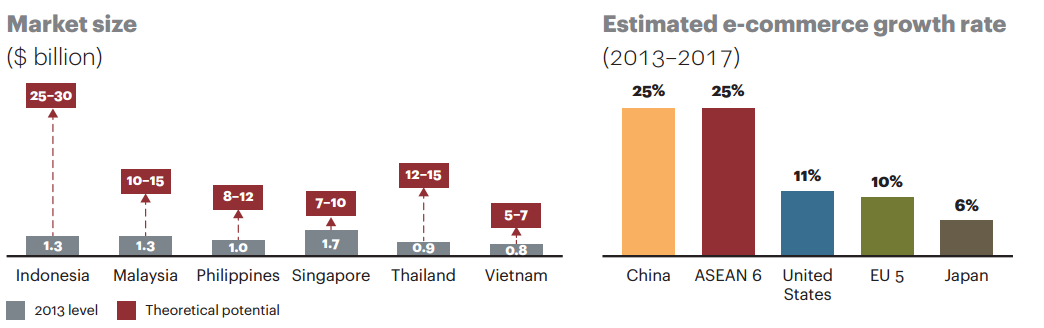
\includegraphics[width=\columnwidth]{figure/marketpotency}
\caption{ASEAN's Market Potency}
\label{market_potency}
\end{figure}

Based on those potential value, Indonesia has many E-commerce companies such as Tokopedia, Bukalapak, Hijup, MatahaMall, etc. This condition make every company must give better service than other. Customer segmentation is one of the way which help companies in understanding customer behavior so that service for the customer can be better.

Data mining can use by company to process data and get customer segmentation. Data mining is techniques for extracting pattern from the data so can get the insight from the data.

Clustering is one of the data mining technique to group objects based on characteristic. Therefore companies can use clustering to perform customer segmentation by grouping objects based on characteristic such as demography, buying patterns, etc.

Community detection is to partition the set of network nodes into multiple groups such that the nodes within a group are connected densely, but connections between groups are sparse.

In this research, we have use another approach, like integrated community detection and clustering to get customer segmentation. This approach applied by detect community based interaction pattern each customer and use clustering with RFM model to get segment from customer have community.



\section{Related Work}
There are some research about customer segmentation. Customer segmentation with RFM model for measure customer loyalty, proposed by Bunnak, Thammaboosadee, dan Kiattisin, they use K-Means and Decision tree to segmenting the customers[1]. Customer segmentation using decision tree to identify VIP customer in mobile communication industry by Zhang Yihua[2].There are some research about community detection. The Girvan-Newman (GN) algorithm proposed by Girvan and Newman [3] exploits the concept of edge betweenness, which is a measure of the centrality and influence of an edge in a network. Community detection in weighted graph based on twitter data use GN algorithm by Mairisha [4]. Based on all research, there is no research about customer segmentation with additional information about community based on customer interaction

\section{Methodology}
In this paper, we apply customer segmentation combine with community detection. The steps of the research process as shown in Fig. 2.

\begin{figure}[h]
\centering
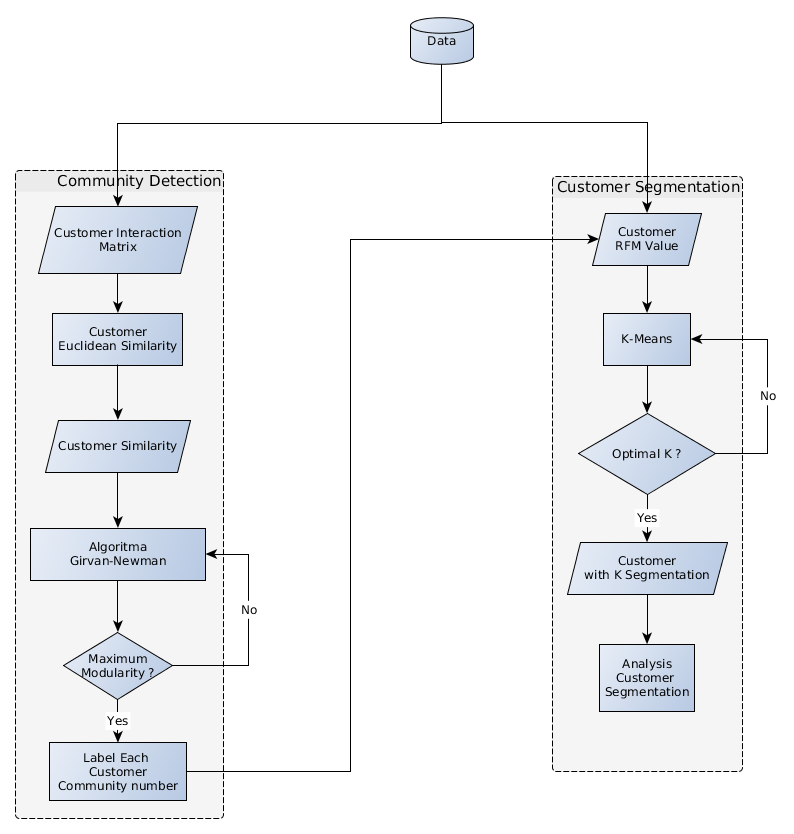
\includegraphics[width=\columnwidth]{figure/overall_methodology}
\caption{Overall methodology}
\label{overall_methodology}
\end{figure}

\subsection{Data and Data Preprocessing}
This step selects related dataset to be used in case study of customer segmentation and then pre-processes data which is an important step. Data preprocessing eliminates irrelevant data by some methods such as data integration, data transformation, and data reduction.

\subsection{Customer Similarity}
In this step, customer similarity is process to find similar from two object. In this research we use euclidean similarity which is common measure [5]. Similarity value from two object become input for next step.

\begin{equation}
    \label{eq:euclidean_distance}
    d( p1,p2 ) = \sqrt{ \Sigma( s_{p1}-s_{p2})^{2} }
\end{equation}
\begin{equation}
	\label{eq:euclidean_similarity}
    \frac{1}{1 + d(p1,p2)}
\end{equation}

\subsection{Community Detection by GN Algorithm}
The GN algorithm is a divisive hierarchical clustering algorithm exploiting the concept of edge betweenness [3]. Three methods were proposed for the calculation of edge betweenness. Among them, the shortest-path method typically shows the best results. The edge betweenness of an edge is informally the number of shortest paths between pairs of nodes that pass through it. Since communities are loosely connected by a few “intergroup” edges, all shortest paths between different communities must pass through one of these few edges. Then, those edges connecting communities will have high edge betweenness. Thus, the communities are detected by eliminating such edges repeatedly.

To decide how much community divide in networks, measure of quality of divide in networks, which  call the modularity. The modularity is, up to a multiplicative constant, the number of edges falling within groups minus the expected number in an equivalent network with edges placed at random, equation (3) show formula from modularity GN [3]

\begin{equation}
	\label{eq:modularity_GN}
    Q = \frac{1}{2m} \Sigma_{vw} [A_{vw} - \frac{(k_{v}k_{w})}{2m}] \sigma(c_{v}c_{w})
\end{equation}

Good community detection on graph have big modularity score, otherwise poor community detection have small modularity score. Modularity score calculate on every create new community. If formed x community, than there is x modularity score. The number of communities that have the highest modularity score indicates the formation of the community in accordance with the actual reality.


\subsection{Customer RFM Model}
In this step, Customer RFM Model is applied by defining the scaling of R, F, and M variable. The
variable is : Recency (R) is customer's last purchase,
Frequency (F) is the total number of purchase during a spesific
period and Monitary (M) is the amount of money used to
purchases in during a spesific period. The RFM model usually
used in retail company. For example the RFM value of
customer in a supermarket, R is the latest time of a customer
purchase, F is how many times a customer made a purchase, and M is how much money that customer have spent [6]. The process of normalization is done for the value of RFM with a range of 1-5 for each customer. Fig 3 is example of RFM Model before transformation and Fig 4 example of RFM Model after transformation

\begin{figure}[h]
\centering
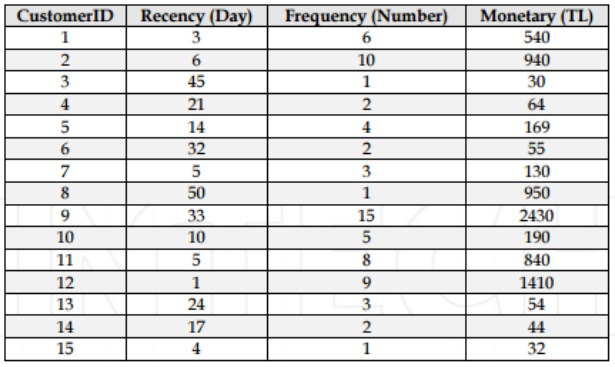
\includegraphics[width=\columnwidth, height=3cm,keepaspectratio]{figure/rfm_model}
\caption{RFM Model before Transformation}
\label{rfm_model}
\end{figure}

\begin{figure}[h]
\centering
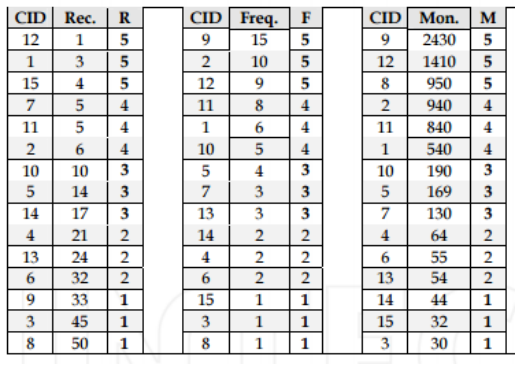
\includegraphics[width=\columnwidth, height=3cm,keepaspectratio]{figure/rfm_model_after}
\caption{RFM Model after Transformation}
\label{rfm_model_after}
\end{figure}

\subsection{Customer Segment by K-Means}
In this step, customer segment is applied by use clustering K-Means algorithm to` find segment each customer. K-Means Clustering is the simplest clustering algorithm. K-means grouped the objects into K clusters. K is the number of clusters that will be generated, defined by the user. The quality of cluster is measured by silhouete. Silhouette can be used to measure the separation distance between the resulting clusters. This measure has a range of [-1, 1]. Step in K-Means Clustering Algorithm is :
\begin{enumerate}
	\item Decide the number of clusters k
	\item Initialize the center of the clusters
	\item Attribute the closest cluster to each data point
	\item Set the position of each cluster to the mean of all data points belonging to that cluster
	\item Repeat steps 3-4 until convergence
\end{enumerate}


\subsection{Analysis Customer Segment}
This step refers to the representation and applying the obtained model to the real usage, which will be discussed in the next section.

\section{Experimental Result}
As described in the previous section, we will organize the experiment results follows with the step of methodology in the previous section.

\subsection{Data and Data Preprocessing}
This research used database from one e-commerce muslimah in Indonesia for last 5 years (2011-2016). The database contains two parts as follows:

\begin{itemize}
	\item Data Interaction 88,103 records
	\item Transaction of customer purchases are total 128,628 records
\end{itemize}

After making a selection of data, the records which include missing values and inaccurate values are removed, and eliminated the redundant attributes. Next, the data is transformed into appropriate formats. Finally, the dataset which are characterized by the following three fields: ID-Sender, ID-Receiver, Total Frequency Interaction

\begin{table}[h]
\renewcommand{\arraystretch}{1.3}
\caption{Sample Data Preprocessing Result}
\label{tab:sample_data_preprocessing_result}
\centering
\begin{tabular}{c|c|c}
    \hline
    ID-Sender  &  ID-Receiver & Total Frequency Interaction\\
    \hline
    79424 & 78112 & 2\\
    \hline
    64554 & 43874 & 2\\
    \hline
    48249 & 21061 & 18\\
    \hline
\end{tabular}
\end{table}

\subsection{Customer Similarity}
In this steps applied formula (2) for data preprocessing result to get similarity each customer based on interaction, table II show sample customer similarity

\begin{table}[h]
\renewcommand{\arraystretch}{1.3}
\caption{Sample Customer Similarity}
\label{tab:sample_customer_similarity}
\centering
\begin{tabular}{c|c|c}
    \hline
    ID-Customer  &  ID-Customer & Similarity\\
    \hline
    38 & 28996 & 0.333333333333\\
    \hline
    21061 & 48249 & 0.0526315789474\\
    \hline
    26797 & 39713 & 0.5\\
    \hline
    33892 & 86097 & 0.333333333333\\
    \hline
\end{tabular}
\end{table}

\subsection{Community Detection by GN Algorithm}
Customer similarity become input for community detection process based on GN Algorithm. Fig 5 show graph based on customer interaction

\begin{figure}[h]
\centering
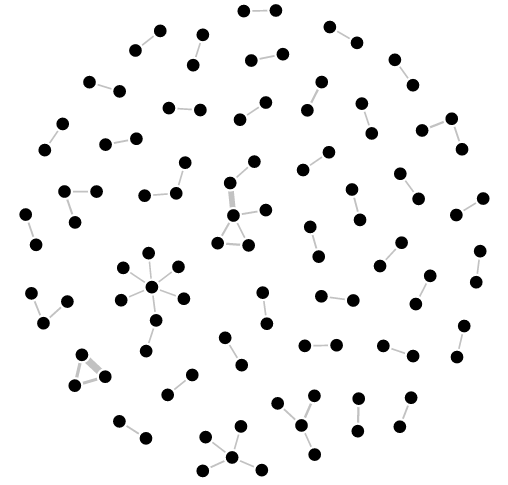
\includegraphics[width=\columnwidth, height=3cm,keepaspectratio]{figure/graph_awal}
\caption{Graph Customer Interaction}
\label{graph_customer}
\end{figure}

For each community detection process iteration, modularity score become quality measure. Table III show modularity score for each number of community formed. Fig 6 show graph result community detection

\begin{table}[h]
\renewcommand{\arraystretch}{1.3}
\caption{Modularity Score}
\label{tab:modularity_score}
\centering
\begin{tabular}{c|c}
    \hline
    Modularity Score  &  Number of Communities\\
    \hline
    0.938736 & 41\\
    \hline
    0.940306 & 42\\
    \hline
    0.844997 & 47\\
    \hline
    0.796996 & 51\\
    \hline
    0.707456 & 56\\
    \hline
\end{tabular}
\end{table}

\begin{figure}[h]
\centering
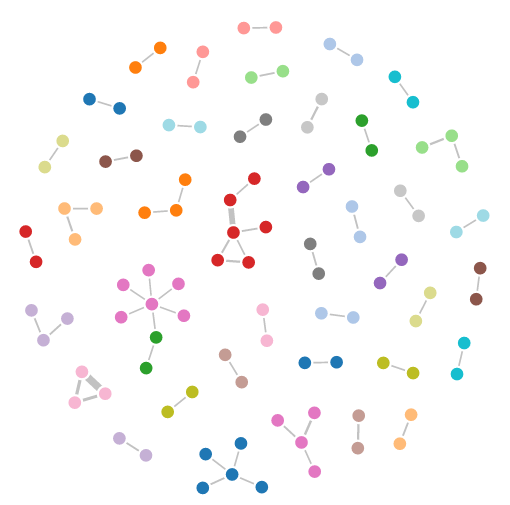
\includegraphics[width=\columnwidth, height=3cm,keepaspectratio]{figure/graph_deteksi}
\caption{Graph Result Community Detection}
\label{graph_community_detection}
\end{figure}

\subsection{Customer RFM Model}
This step uses data obtained in the previous step applied with the defined the scales of R, F, M attributes as described in the previous section.

\subsection{Customer Segment by K-Means}
In this process, customer are classified by K-Means based on RFM value and use K range of [3-8]. With silhouete score, K cluster with best silhouete score is choosen to become number of segments formed. Table IV show silhouete score each K cluster.

\begin{table}[h]
\renewcommand{\arraystretch}{1.3}
\caption{Result K-Means with Silhouete Score}
\label{tab:result_k-means}
\centering
\begin{tabular}{c|c}
    \hline
    Number of Cluster & Silhouete Score\\
    \hline
    3 & 0.407802895718\\
    \hline
    4 & 0.405678928295\\
    \hline
    5 & 0.40253003193\\
    \hline
    6 & 0.415421594014\\
    \hline
    7 & 0.408311013086\\
    \hline
    8 & 0.402908225812\\
    \hline
\end{tabular}
\end{table}

6 Cluster have best silhouete score, than customer segment divided into 6 segment. Centroid each cluster is used to know characteristic for each cluster formed. Table V show centroid for 6 cluster. 

\begin{table}[h]
\renewcommand{\arraystretch}{1.3}
\caption{Centroid Cluster}
\label{tab:centroid_cluster}
\centering
\begin{tabular}{c|c|c|c}
    \hline
    Cluster & Recency & Frequency & Monetary\\
    \hline
    1 & 2.15384615 & 1.61538462 & 1.53846154\\
    \hline
    2 & 1.2 & 4.8 & 4.86666667\\
    \hline
    3 & 4.52941176 & 2.35294118 & 2.52941176\\
    \hline
    4 & 2.10526316 & 3.15789474 & 3.21052632\\
    \hline
    5 & 3.52941176 & 4.41176471 & 4.29411765\\
    \hline
    6 & 4.69230769 & 1.07692308 & 1.07692308\\
    \hline
\end{tabular}
\end{table}

\begin{table}[h]
\renewcommand{\arraystretch}{1.3}
\caption{Result Customer Segmentation}
\label{tab:result_all}
\centering
\begin{tabular}{c|c|c}
    \hline
    ID-Customer & Cluster & Community\\
    \hline
    29167 & 5 & 7\\
    \hline
    26797 & 2 & 14\\
    \hline
    33548 & 2 & 14\\
    \hline
    65182 & 2 & 33\\
    \hline
\end{tabular}
\end{table}

In addition to successful classify customers into each segments, there is also relevant information for every member of the community formed segment. Such information can help e-commerce in developing marketing strategies for each segment, because that information can develop more specific strategies.



\subsection{Analysis Customer Segment}
By knowing the characteristics of each segment is shown in Table VII and customer segmentation result show on Table VI, the company can provide different treatment to certain customers in the segment. For example in the Loyal Customer Segment, there are some members of that segment is incorporated in the dominant community of its members incorporated herein Profit Customer Segment, so the company can provide different treatment for these customers to be able to increase transactions, thus increasing segment type, of Loyal Customer Segment into Profit Customer Segment.

\begin{table}[h]
\renewcommand{\arraystretch}{1.3}
\caption{Character Segment}
\label{tab:Character_segment}
\centering
\begin{tabular}{c|c|c|c|c}
    \hline
    Cluster & Recency & Frequency & Monetary & Description\\
    \hline
    1 & Low & Low & Low & New Customer\\
    \hline
    2 & Low & High & High & Profit Customer\\
    \hline
    3 & High & Low & Low & Churn Customer\\
    \hline
    4 & Low & Medium & Medium & Loyal Customer\\
    \hline
    5 & Medium & High & High & Profit Customer\\
    \hline
    6 & High & Low & Low & Churn Customer\\
    \hline
\end{tabular}
\end{table}

\section{Conclusion}
This research attemps to try combine community detection and clustering process applying to customer segmentation. This research take RFM model and K-Means Clustering, and use GN algorithm for community detection then the result can be identified characteristics each segment with knowledge about community each segment. It is useful for company to develope specific strategic marketing.




% conference papers do not normally have an appendix


\begin{thebibliography}{1}

\bibitem{IEEEhowto:Bunnak}
Bunnak., Thammaboosadee., and Kiattisin, "Applying Data Mining Techniques
and Extended RFM Model in Customer Loyalty Measurement" Journal of
Advances in Information Technology Vol. 6, No. 4, November 2015

\bibitem{IEEEhowto:Yihua}
Zhang Yihua, "Vip Customer Segmentation Based on Data Mining in
Mobile-communication Industry". IEEE 978-1-4244-6005-2/10, 2010

\bibitem{IEEEhowto:Newman}
M. E. Newman and M. Girvan, "Finding and evaluating
community structure in networks," Physical Review E,
vol. 69, no. 2, p. 026113, 2004.

\bibitem{IEEEhowto:Mairisha}
Mairisha, M, "Integration of Coupling Degree Concept for Calculating Modularity in Quality Analysis of
Community Structure Based on Weighted Graph" Master’s Program Thesis, Institut Teknologi Bandung, 2016

\bibitem{IEEEhowto:Segaran}
Segaran, T, "Programming Collective Intelligence", O'Reilly Press 2007

\bibitem{IEEEhowto:Tsiptsis}
Tsiptsis, K., and Chorianopoulos, A, "Data Mining Techniques in CRM", Wiley 2009
\end{thebibliography}




% that's all folks
\end{document}


